\chapter{Uživatelská příručka}

Obrázek \ref{img:hp} ukazuje Homepage projektu.

Uživatel může do textového pole zadávat požadované dotazy, hned vedle se nalézá tlačítko pro vyhledání dotazu.

Nad vyhledávacím polem je umístěna základní navigace, která slouží pro přepínání mezi druhy dotazů.

\begin{figure}[h]
\begin{center}
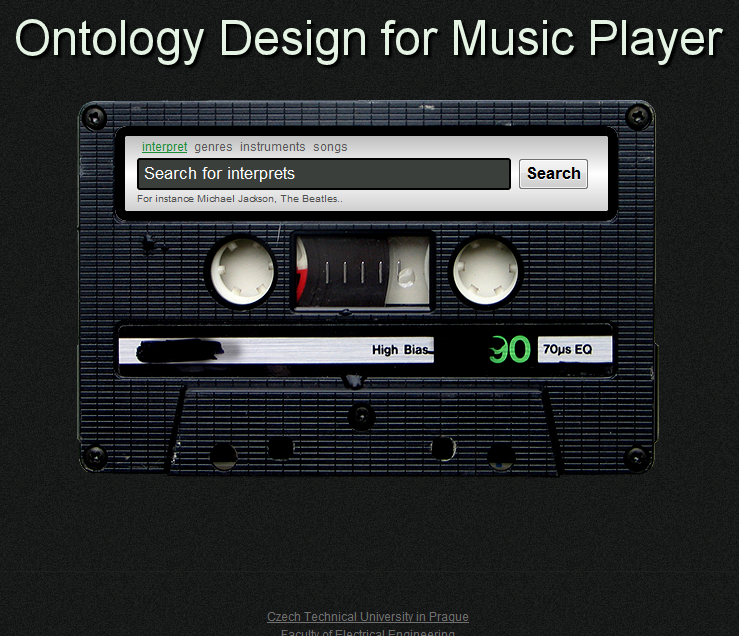
\includegraphics[width=15cm]{figures/hp}
\caption{Výřez homepage projektu}
\label{img:hp}
\end{center}
\end{figure}

Na stránce s výsledky jsou pod vyhledávacím formulářem umístěny výsledky hledání (viz obr \ref{img:searchresults}). Každý výsledek je ve formě hypertextového odkazu, vedoucí na patřičnou stránku.

\begin{figure}[h]
\begin{center}
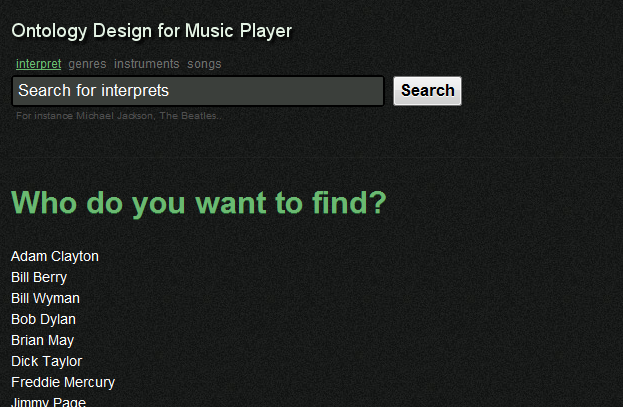
\includegraphics[width=14cm]{figures/searchresults}
\caption{Výřez stránky s výsledky}
\label{img:searchresults}
\end{center}
\end{figure}

V patičce jsou umístěny informace o autorovi projektu.